Traditionnellement, nous étudions les variations de la fonction
$A(x) = x f(x) = \frac{7 x - x^2}{x + 2}$, via sa dérivée
$\sder{A}{1}(x) = \frac{- x^2 - 4 x + 14}{(x + 2)^2}$, dont le signe dépend de celui du trinôme $T(x) = - x^2 - 4 x + 14$ qui s'annule en $\big( - 2 \pm 3 \sqrt{2} \big)$.
Nous obtenons aisément le tableau de variations suivant.
%
\begin{center}
	\begin{tikzpicture}
                \tkzTabInit[espcl=2.5]{
                	$x$              / 1    ,
    				$T(x)$           / 1.25 ,
    				$\sder{A}{1}(x)$ / 1    ,
    				$A(x)$           / 1.5
    			}{$0$, $3 \sqrt{2} - 2$, $7$}
    
                \tkzTabLine{ t , + , z , - , }
                \tkzTabLine{ t , + , z , - , }

                \tkzTabVar{-/ , +/, -/ }
	\end{tikzpicture}
\end{center}


Finalement,
$\area(MNOP)$ est maximale uniquement lorsque $x_M = 3 \sqrt{2} - 2$.


\begin{remark}
	Comme
	$\sder{A}{2}(x) = - \frac{36}{(2 + x)^3}$,
	la fonction $A$ est concave.
\end{remark}
